%less comparisions, logarithmic stuff, etc.

Da sich während des Prozess der Labelgeneration und Konfliktermittlung die Positionen der Knoten nicht verändern, wäre es sehr ineffizient,
immer wieder alle Knoten (und deren Labels, sofern generiert) abzufragen.

Da die Aufteilung der Knoten im Raum gleich bleibt (innerhalb einer Iteration des Render-Loops), ist es sinnvoller, diese einmalig zu Beginn
in einem Quadtree zu sortieren bzw. zu strukturieren.

Im Vergleich zu der naiven Methode mit einer Komplexität von $O(n^2)$ (da $n$-mal Knoten mit $n-1$ anderen Knoten verglichen werden) befindet man sich mit dem Quadtree in der Komplexitätsklasse
$O(n \log n)$\footnote{ Vorausgesetzung: Der Baum ist gut balanciert}\cite{quadtree}.

Das Vorgehen des Quadtrees ist simpel: Initial startet man mit dem gesamten Bildschirm und allen Knoten.
Nun ermittelt man den Mittelwert der $x$-Werte der Knoten und dasselbe analog für die $y$-Werte.
Diese beiden Mittelwerte teilen nun als Geraden den Bildschirm in vier nicht zwangsläufig gleich große Teilbereiche.

Diese Teilbereiche haben annähernd die gleiche Anzahl an Knoten, im Idealfall $\frac{n}{4}$ der Knoten des Gesamtbereiches.
Nun wird für diese Teilbereiche rekursiv das gleiche Verfahren angewandt wie eben für den gesamten Bildschirm beschrieben.
Rekursionsabbruch ist, wenn die Teilbereiche weniger als zwei Knoten enthalten oder die maximale Rekursionstiefe erreicht ist (siehe \hyperref[sec:consts]{Magic Constants}).

Ein Sonderfall stellen Knoten dar, durch die die Trenngerade der Bereiche verläuft (da es sich hier nicht um Punkte handelt).
Diese müssen dann in beiden Teilbereichen, auf jeder Seite der Trenngerade, als enthalten gezählt werden.

Das ist eine Schwachstelle des Quadtree in Situation, in denen die Knoten sehr stark aufeinander sind,
z. B. bei starkem Zoom Out oder wenn die Lens Funktion von \texttt{iGraph.js} verwendet wird.

Da die Knoten dann fast identische Positionen haben, gelingt keine Aufteilung der Knoten in Teilregionen und alle Knoten sind in nahezu allen Regionen.
Das führt den logarithmischen Charakter des Baums ad absurdum.

Der Quadtree erkennt selbst anhand eines Grenzwertes (\hyperref[sec:consts]{Magic Constants}), ob er ineffizient ist.
Eine Lösung dafür wird ist ein \hyperref[subsec:zoom]{Zoom Mode}, der nachfolgend erklärt wird.
Sollte auch das nicht möglich sein, werden die Knoten in den ineffizienten Teilregionen (also die den Grenzwerte von $x$ Elementen pro Teilregion überschreiten) selbst als ineffizient markiert
und werden beim Labeling übersprungen (obwohl sie sichtbar sind). Die Chance, die freie Kapazität bis zur Maximalanzahl an gezeigten Labels zu nutzen,
wird dann anderen, weniger relevanten (laut Vorsortierung), dafür effizienten Knoten gelassen.

In den meisten Fällen ist der Quadtree aber effizient und das Ergebnis sind viele kleine, unabhängige Teilbereiche, in denen nur sehr wenige Knoten enthalten sind.
Wenn nun ein potenzielles Label überprüft werden soll, so wird geguckt, welche Teilregionen des Quadtrees es überdeckt.

\begin{figure}[H]
    \centering
    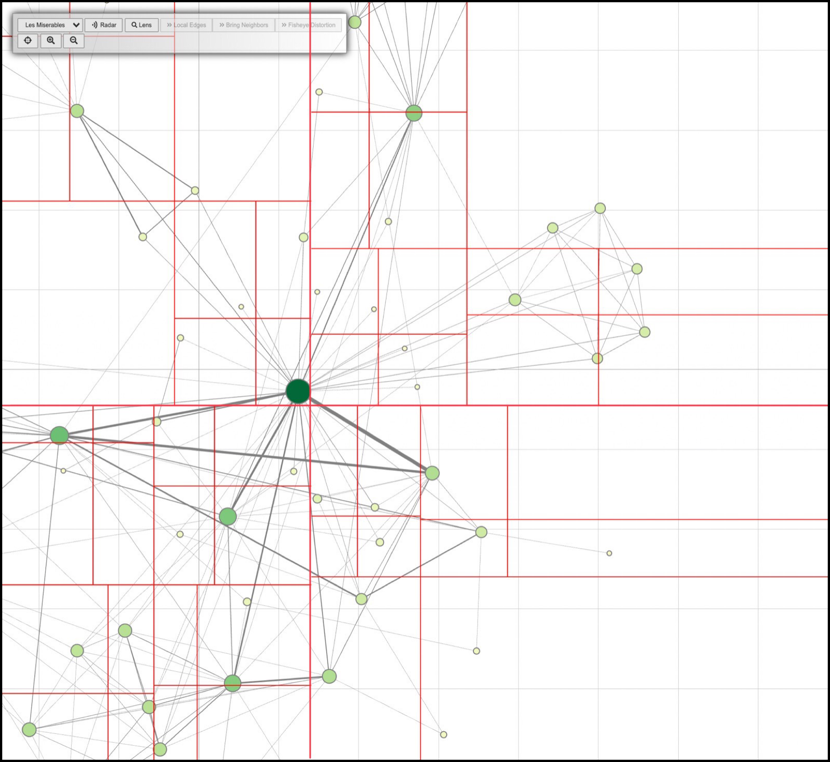
\includegraphics[scale=0.33]{../img/quadtree}
    \caption{Aufteilung eines Quadtrees in seine Teilbereiche}
    \label{fig:quadtree}
\end{figure}

Mit allen Knoten, die in diesen überdeckten Regionen enthalten sind, wird dann eine individuelle Konfliktermittlung durchgeführt.
Das heißt, es werden nur Konflikte in der Nähe der potenziellen Labelposition direkt kontrolliert und der Rest wurde eliminiert
durch den rekursiven Abstieg (mit Zugriffszeit $O (\log n)$) im Quadtree mit Grenzen, also der Bounding Box, des Labels.

Bleibt die potenzielle Labelposition (nach der Beschreibung aus \hyperref[subsubsec:label_conflict]{Label Conflicts} mit allen Elementen der überdecken Teilbereiche) konfliktfrei,
so kann es zu einem tatsächlichen Label gemacht werden.
Dieses wird als neues Element in die eben überprüften Teilregionen übernommen, sodass es zukünftig auch im Quadtree repräsentiert ist und bei der Konfliktermittlung berücksichtigt wird.



